
%%%%%%%%%%%%%%%%%%%%%%% file typeinst.tex %%%%%%%%%%%%%%%%%%%%%%%%%
%
% This is the LaTeX source for the instructions to authors using
% the LaTeX document class 'llncs.cls' for contributions to
% the Lecture Notes in Computer Sciences series.
% http://www.springer.com/lncs       Springer Heidelberg 2006/05/04
%
% It may be used as a template for your own input - copy it
% to a new file with a new name and use it as the basis
% for your article.
%
% NB: the document class 'llncs' has its own and detailed documentation, see
% ftp://ftp.springer.de/data/pubftp/pub/tex/latex/llncs/latex2e/llncsdoc.pdf
%
%%%%%%%%%%%%%%%%%%%%%%%%%%%%%%%%%%%%%%%%%%%%%%%%%%%%%%%%%%%%%%%%%%%


\documentclass[runningheads,a4paper]{llncs}

\usepackage[T5]{fontenc}
\usepackage[utf8]{inputenc}

\usepackage{amssymb}
\setcounter{tocdepth}{3}
\usepackage{graphicx}
\usepackage{epstopdf}
\usepackage{url}
\usepackage{array}
\usepackage{multirow}
\usepackage{booktabs}
\usepackage{array}
\usepackage{caption} 
%\usepackage{amsmath}
\newcolumntype{L}[1]{>{\raggedright\let\newline\\\arraybackslash\hspace{0pt}}m{#1}}
\newcolumntype{C}[1]{>{\centering\let\newline\\\arraybackslash\hspace{0pt}}m{#1}}
\newcolumntype{R}[1]{>{\raggedleft\let\newline\\\arraybackslash\hspace{0pt}}m{#1}}

% \preto\tabular{\setcounter{magicrownumbers}{0}}
% \newcounter{magicrownumbers}
% \newcommand\rownumber{\stepcounter{magicrownumbers}\arabic{magicrownumbers}}
\urldef{\mailsa}\path|{1212304,1212069}@student.hcmus.edu.vn, nqminh@fit.hcmus.edu.vn|
%\bibliography{typeinst}
%\urldef{\mailsa}\path|{alfred.hofmann, ursula.barth, ingrid.haas, frank.holzwarth,|
%\urldef{\mailsb}\path|anna.kramer, leonie.kunz, christine.reiss, nicole.sator,|
%\urldef{\mailsc}\path|erika.siebert-cole, peter.strasser, lncs}@springer.com|    
% \newcommand{\keywords}[1]{\par\addvspace\baselineskip
% \noindent\keywordname\enspace\ignorespaces#1}
% \graphicspath{ {images/} }

\begin{document}

\mainmatter  % start of an individual contribution

% first the title is needed
\title{Lifelong learning for cross-domain Vietnamese sentiment classification}

% a short form should be given in case it is too long for the running head
\titlerunning{Lifelong learning for cross-domain Vietnamese sentiment classification}

% the name(s) of the author(s) follow(s) next
%
% NB: Chinese authors should write their first names(s) in front of
% their surnames. This ensures that the names appear correctly in
% the running heads and the author index.
%
\author{Quang-Vinh Ha
	\and Bao-Dai Nguyen-Hoang
	\and Minh-Quoc Nghiem}
\institute{Faculty of Information Technology\\
	Ho Chi Minh City University of Science\\
	227 Nguyen Van Cu St., Ward 4, District 5, Ho Chi Minh City, Vietnam\\
\mailsa
}

%\thanks{Please note that the LNCS Editorial assumes that all authors have used
%the western naming convention, with given names preceding surnames. This determines
%the structure of the names in the running heads and the author index.}%

%

% (feature abused for this document to repeat the title also on left hand pages)

% the affiliations are given next; don't give your e-mail address
% unless you accept that it will be published

%\mailsa\\
%\mailsb\\
%\mailsc\\
%\url{http://www.springer.com/lncs}}

%
% NB: a more complex sample for affiliations and the mapping to the
% corresponding authors can be found in the file "llncs.dem"
% (search for the string "\mainmatter" where a contribution starts).
% "llncs.dem" accompanies the document class "llncs.cls".
%

\toctitle{Lifelong learning for cross-domain Vietnamese sentiment classification}
%\tocauthor{Authors' Instructions}
\maketitle


\begin{abstract}
This paper proposes an improvement to lifelong learning for cross-domain sentiment classification.
Lifelong learning is to retain knowledge from past learning tasks to improve the learning task on a new domain.
In this paper, we will discuss how bigram and bag-of-bigram features integrated into a lifelong learning system can help improve the performance of sentiment classification on both Vietnamese and English.
Also, pre-processing techniques specifically for our cross-domain, Vietnamese dataset will be discussed.
Experimental results show that our method achieves improvements over prior systems and its potential for cross-domain sentiment classification.
%Statistical machine learning techniques have achieved promising results for sentiment classification.
%In the Internet age, it is essential to transfer the knowledge from the domain we learned to adapt an unfamiliar domain and still have a high accuracy of predicting if a user review is positive or negative.
%lifelong learning had proved its performance in topic modeling and sentiment classification in English.
%However, for low-resource language such as Vietnamese, there are many problems to deal with to get the similar performance.
%This paper presents an empirical study on Vietnamese sentiment classification.
%Our proposed method is based on lifelong learning but combined with black-list and segmentation techniques specifically for Vietnamese.
%The results are promising, showing that the method is able to make relatively accurate predictions even when no labeled data is given.

\keywords{sentiment classification; Vietnamese; supervised learning, lifelong learning}
\end{abstract}

\section{Introduction}
%
%
%

%propose the use of bi-gram
%contribution

% RULE: Topic sentence at the beginning of the paragraph

% OK: importance of sentiment analysis and sentiment classification, focus of this paper 
The rapid growth of e-commerce and the Web age quickly makes the sentiment knowledge become an advantage to contribute more values to market predictions.
Sentiment analysis remains a popular topic for research and developing sentiment-aware applications~\cite{Pang08opinionmining}.
Sentiment classification, which is a subproblem of sentiment analysis task, is the task of classifying whether an evaluative text is expressing a positive, negative or neutral sentiment.
In this paper, we focus on document-level binary sentiment classification, in which the sentiment is either positive or negative.

% OK: Intro transfer learning, multi-domain classification, lifelong learning
In recent years, most studies on sentiment classification adopt machine learning and statistical approaches~\cite{Liu12sentimentanalysis}.
Such approaches hardly perform well on real-life data, which contains opinionated documents from domains different from the domain used to train the classifier.
To overcome this limitation, lifelong learning~\cite{chen-ma-liu:2015:ACL-IJCNLP}, transfer learning~\cite{Pan:2010:STL:1850483.1850545}, self-taught learning~\cite{Raina:2007:SLT:1273496.1273592} and other domain adaptation techniques~\cite{Pan:2010:STL:1850483.1850545} were proposed.
All mentioned methods is to transfer the knowledge gained from source domains to improve the learning task on the target domain.

% lifelong learning, drawbacks: unigram --> Vietnamese
Chen et al.~\cite{chen-ma-liu:2015:ACL-IJCNLP} proposed a novel approach of lifelong learning for sentiment classification, which is based on Naïve Bayesian framework and stochastic gradient descent.
Although this approach could deal with cross-domain sentiment classification, it used the ``bag-of-words'' model and faces difficulties when represent the relationship between words.
For example, the phrase ``have to'', which is a common phrase in the negative text (but much less important in positive text), cannot be taken advantage of with bag-of-words feature.
This is especially true in isolated languages, such as Vietnamese, where words are not separated by white spaces.

%Vietnamese, no domain adaptation, no transfer learning
As a resource-poor language, Vietnamese has quite a few accomplishments in the field of sentiment classification.
To the best of our knowledge, there is no study on Vietnamese cross-domain sentiment classification.
There is also no suitable dataset with a reasonable amount of reviews and variance of products to apply lifelong learning on Vietnamese.

%propose the use of bi-gram
%contribution
In this paper, we propose the use of bi-gram feature to lifelong learning approach on sentiment classification.
Wang and Manning~\cite{wang-manning:2012:ACL2012short} proved that adding bi-grams improves sentiment classification performance because they can capture modified verbs and nouns.
We also created a dataset for Vietnamese cross-domain sentiment classification by collecting more than 15,000 reviews from the e-commerce website Tiki.vn~\footnote{http://tiki.vn/} with 17 distinctive domains.
We proposed combining the bi-gram feature with the Naïve Bayesian optimization framework.
The proposed method has leveraged the phrases that contain sentiment better than that of Chen et al.~\cite{chen-ma-liu:2015:ACL-IJCNLP} and outperforms other methods in both Vietnamese and English datasets.

% SHORT thêm reading guide
The remainder of this paper is organized as follows.
Section 2 provides a brief overview of the background and related work.
Section 3 presents our method including how we add bi-gram and bag-of-bi-gram features to the lifelong learning, and how we processed the raw reviews of the Vietnamese dataset to improve the performance.
Section 4 describes the experimental setup and results.
Section 5 concludes the paper and points to avenues for future work.



%NOTE: 2 tac gia: A and B~\cite{}
% 3 tac gia tro len: A et al.~\cite{}
% Khong de nam, vd nhu vay la ko duoc: A 2015~\cite{}
% Neu su dung thi` present thi du`ng present luon, neu du`ng past thi du`ng past luon

\section{Related Work}
%Vietnamese Sentiment classification, lifelong learning, 
Our work is related to lifelong learning, multi-task learning, transfer learning and domain adaptation.
Chen and Liu have exploited different types of knowledge for lifelong learning on mining topics in documents and topic modeling~\cite{chen2014mining,icml2014c2_chenf14}.
Chen and Liu~\cite{chen-ma-liu:2015:ACL-IJCNLP}, in their other work, also proposed the first lifelong learning approach for sentiment classification.
Likewise, Ruvolo and Eaton~\cite{ruvolo2013scalable} developed a method for online multi-task learning in the lifelong learning setting, which maintains a sparsely shared basis for all task models.
About domain adaptation, most of the work can be divided into two groups: supervised (Finkel and Manning 2009~\cite{Finkel:2009:HBD:1620754.1620842}, Chen et al. 2011~\cite{chen2011co}) and semi-supervised (Kumar et al. 2010~\cite{kumar2010co}, Huang and Yates 2010~\cite{huang2010exploring}).

There are also many previous works on transfer learning and domain adaptation for sentiment classification.
Yang et al.~\cite{yang2006knowledge} proposed an approach based on feature-selection for cross-domain sentence-level classification.
Other approaches include structural correspondence learning (Blitzer et al.~\cite{blitzer2007biographies}), spectral feature alignment algorithm (Pan et al. 2010~\cite{pan2010cross}), CLF (Li and Zong 2008~\cite{li2008multi}).
Similar methods can be found in the work of Liu~\cite{Liu12sentimentanalysis}.
%there must be something wrong with other approaches

In the field of sentiment analysis for Vietnamese, Duyen et al.~\cite{Duyen-Bach:2014} has published an empirical study which compared the use of Naïve Bayes, MEM and SVM with hotel reviews.
Also, using the corpus from Duyen, Bach et al.~\cite{Bach2015322} proposed the use of user-ratings for the task.
Term feature selection approach was investigated by Tran et al. 2011~\cite{zhang2011information}, while Kieu and Pham~\cite{kieu2010sentiment} investigated a rule-based system for Vietnamese sentiment classification.
As that being said, to the best of our knowledge, there is no previous work on domain adaptation or lifelong learning as well as a appropriate dataset for Vietnamese (with a reasonable amount of reviews and variance of products).

\section{Our Proposed Method}

%overview
In this section, we describe our system for sentiment classification in a lifelong learning setting, which is a combination of components to analyze reviews from many domains.
The system takes customer reviews, from multiple types of products, as source domains.
Each review can contain multiple sentences and it is labeled positive, negative or neutral based on how users rated them.
From the source domains mentioned above, the system gains knowledge valuable to the learning task on the target domain.
Such knowledge is used to optimize the classifier on the target domain using stochastic gradient descent (SGD).
          
%như title
\subsection{Overview of lifelong learning for sentiment classification}
As described in figure~\ref{figure: LLL}, the system contains three main modules: knowledge storing, optimization, and sentiment classification.

\begin{figure}
	\centering                                    
	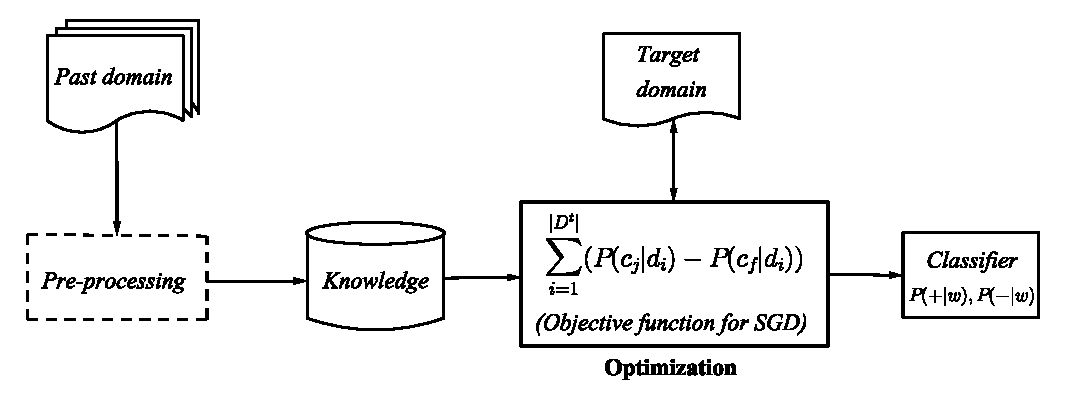
\includegraphics[height=4.35cm]{process_vector}
	\caption{Lifelong learning for sentiment classification}
	\label{figure: LLL}
\end{figure}

\subsubsection{Knowledge storing}
The system extracts knowledge from the past domains, which is used to optimize the classifier on the target domain.
There are three types of knowledge, including:
%do the reviewers have to know these?
\begin{itemize}
	\item
	The Prior probability $P^t_+(w|c)$ and $P^t_-(w|c)$ of each word, where t is a past learning task.
	%Because we choose to combine Naïve Bayes and bigram feature, $
	\item
	Number of times a word appears in positive or negative in learning task: $N^t_{+,w}$, $N^t_{-,w}$.
	Similarly, the number of occurrences of $w$ in the positive and negative documents are respectively $N^{KB}_{+,w}= \sum{N^t_+}$ and $N^{KB}_{-,w} = \sum{N^t_-}$
	\item
	Number of past tasks in which $P_{w|+}>P_{w|-}$ or vice versa: $M^{KB}_{+,w}$, $M^{KB}_{-,w}$.
	The two figures are used to leverage domain knowledge via a penalty term to penalize the words that appear in just a few domains. %less than a reasonable number of domains
\end{itemize}

\subsubsection{Optimization}
With the help of all three types of knowledge mentioned above, this component is used to optimize the objective function on the training set of the target domain. %to get the most optimized classifier for testing.
The objective function is $\sum_{i=1}^{|D_i|}{P(c_j|d_i)-P(c_f|d_i)} $ , in which $c_j$ is the actual labeled class, $c_f$ is the wrong class of the document $d_i$.
We follow the SGD with similar regularization techniques proposed by Chen et al.~\cite{chen-ma-liu:2015:ACL-IJCNLP}.
Our optimized variables are $X_{+,w}$ and $X_{-,w}$, which are the occurrences of a word $w$ in a positive and negative class, respectively. 
The objective function is optimized on each document of the target domain until convergence.
After SGD, we use Bayes formula (see equation~\ref{equa:nb+},~\ref{equa:nb-}) to create a classifier optimized for the target domain. 
Note that Laplace smoothing is applied in both cases.
\begin{equation}
P(+|w)= \frac{\lambda + X_{+,w}}{\lambda|V|+\sum_{v=1}^{V}{X_{+,v}}}
\label{equa:nb+}
\end{equation}
\begin{equation}
P(-|w)= \frac{\lambda + X_{-,w}}{\lambda|V|+\sum_{v=1}^{V}{X_{-,v}}}
\label{equa:nb-}
\end{equation}

\subsubsection{Sentiment classification}
With the classifier optimized for the target domain, the system does sentiment classification task on each document of the test domain. 
Although the approach still follows Naïve Bayes framework, the way we classify differentiates between unigrams, bigrams, and bag-of-bigrams.



\subsection{Bigrams}
%bigram illustration
We propose the use of bigram feature, instead of unigram, on this type of sentiment classification.
Wang and Manning~\cite{wang-manning:2012:ACL2012short} has proved that using bigram always improve the performance on sentiment classification.
%Due to the fact that there are a lot of phrases that can express sentiment in the documents, the bigram feature can help improve the original Naive Bayes framework applying unigram feature with classifier 
For instance, phrases such as ``have to'' in English or ``không thích'' (dislike) in Vietnamese can express sentiment well in the documents.
These noun phrases and verb phrases cannot be captured by using unigram feature alone.
%Hence, using bigram feature captures modified and nouns.
%Bigram feature also helps capture (adjective + noun), (verb + adverb).e.g phrases in both Vietnamese and English.
%The modified model we choose to combine Naïve Bayes and bigram feature is described below:

The way we integrate bigram feature into Naïve Bayesian framework for lifelong learning is described below:

\begin{itemize}
	
\item In \textbf{Knowledge storing} step, beside $P^t_+(w|c)$ and $P^t_-(w|c)$, we also store $P^t_+(w_i|w_{i-1})$ and $P^t_-(w_i|w_{i-1})$ whereas $P^t_+(w_{i+1}|w_i) = \frac{\lambda + N_{+,w_iw_{i+1}}}{\lambda|V|+N_{+,w_i}}$ and $P^t_-(w_{i+1}|w_i)= \frac{\lambda + N_{-,w_iw_{i+1}}}{\lambda|V|+N_{-,w_i}}$). 
The number of occurrences of each bigram on each class ($N^t_{+,w_iw_{i+1}}$ and $N^t_{-,w_iw_{i+1}}$) and the domain-level knowledge  ($M^{KB}_{+,w_iw_{i+1}}$, and  $M^{KB}_{-,w_iw_{i+1}}$) are also stored. 
			
\item In \textbf{Optimization} step, due to the use of bigram, the probability for each document is modified as equations~\ref{pdoc+},~\ref{Pdoc-}:
\begin{equation}
P(+|d) = \frac{P_+}{P_-}.P_+(w_0).P_+(w_1|w_0).P_+(w_2|w_1)…P_+(w_n|w_{n-1}) 
\label{pdoc+}
\end{equation}

\begin{equation}
P(-|d) = \frac{P_-}{P_+}.P_-(w_0).P_-(w_1|w_0).P_-(w_2|w_1)…P_-(w_n|w_{n-1}) 
\label{Pdoc-}
\end{equation}

\item The positive and negative probabilities for each document on the test data also have to follow the equations~\ref{pdoc+},~\ref{Pdoc-} for the \textbf{Sentiment Classification} step.

\end{itemize}

\subsection{Bag of bigrams} %better performance, relies on probability of unigram
%bag-of-bigrams illustration
Although using bigram help taking advantage of the phrases that express sentiments, using the standard Bayes formula still relies on the probabilities and number of occurrences of unigrams on all the documents.
Our alternative way to leverage bigram is to treat each bigram as a unigram and apply the normally used Bayes formula ( $P_{+|d} = \frac{P_+}{P_-}.P_+(w_0w_1).P_+(w_1w_2).P_+(w_2w_3)…P_+(w_{n-1}w_n) $) to create the classifier.
Such formula is applied to \textbf{Optimization} and \textbf{Sentiment classification} steps. 
%This bag-of-bigram approach help reduce the size of vocabulary set to contains only bigrams instead of both, which decrease the required time to complete the task.
%In experimental results, we will compare how the two solutions improve the classification performance on both Vietnamese and English dataset.
We will compare how the two solutions improve the classification performance on both Vietnamese and English dataset.

\subsection{Pre-Processing on Vietnamese dataset}
Different to the dataset from Chen et al.~\cite{chen-ma-liu:2015:ACL-IJCNLP} on English, the Tiki.vn dataset contains many emoticons. 
Therefore, we need to pre-process the data before \textbf{Knowledge storing} step to leverage all lexical resources in the dataset. 
In most online forums or discussion groups, users often use emoticons such as ``:)'', ``:('' or punctuations such as ``!!!!!'' to express their opinions.
However, during the task, we standardize the emoticons used by users, e.g. changing ``:((((('' to ``:(''.
We treat each emoticon or punctuation as a unigram and follow the other steps as normal.
%This approach has slightly improved our performance on Vietnamese dataset.
In this pre-processing step, we also perform word segmentation by following the maximum entropy approach of Dinh and Vu~\cite{DDien-VThuy:2006}.
Word segmentation can model the sentiment adjectives which often contain two or more morphemes, hence, provide a better vocabulary set for classification on Vietnamese using unigram feature.

%\item \textbf{Optimization}: This component follow the stochastic gradient descent with similar regularization techniques proposed by Chen et al.~\cite{chen-ma-liu:2015:ACL-IJCNLP}.
%The component will use the knowledge above to update the virtual count $X$ until convergence to get the best classifier for the target domain.
%\item \textbf{Sentiment classification}: With the classifier optimized for the target domain, the system does sentiment classification task on each document of the test domain %To have a truly overall view of lifelong learning for Vietnamese sentiment classification, we test the classifier which is just optimized for the target domain on different cases including segmentation and without segmentation task, unigram feature and bigram feature, with and without stop words.

%This component is to process the reviews, especially the raw reviews of the Vietnamese dataset, in a suitable type.
%%On our dataset, the average unigram per document on each domain varies from 66 to just above 75 unigrams.
%The input collection includes a number of past domains and one target domain.
%The knowledge gained from the input domain will be used to add values to the learning task on the target domain.
%%Finally, with refined parameters, the system will classify reviews on the testing part of the target domain.
%
%The system contains three main modules: storing knowledge, optimization, and sentiment classification.
%
%% Storing knowledge
%
%% optimization
%
%% sentiment classification
%

%
%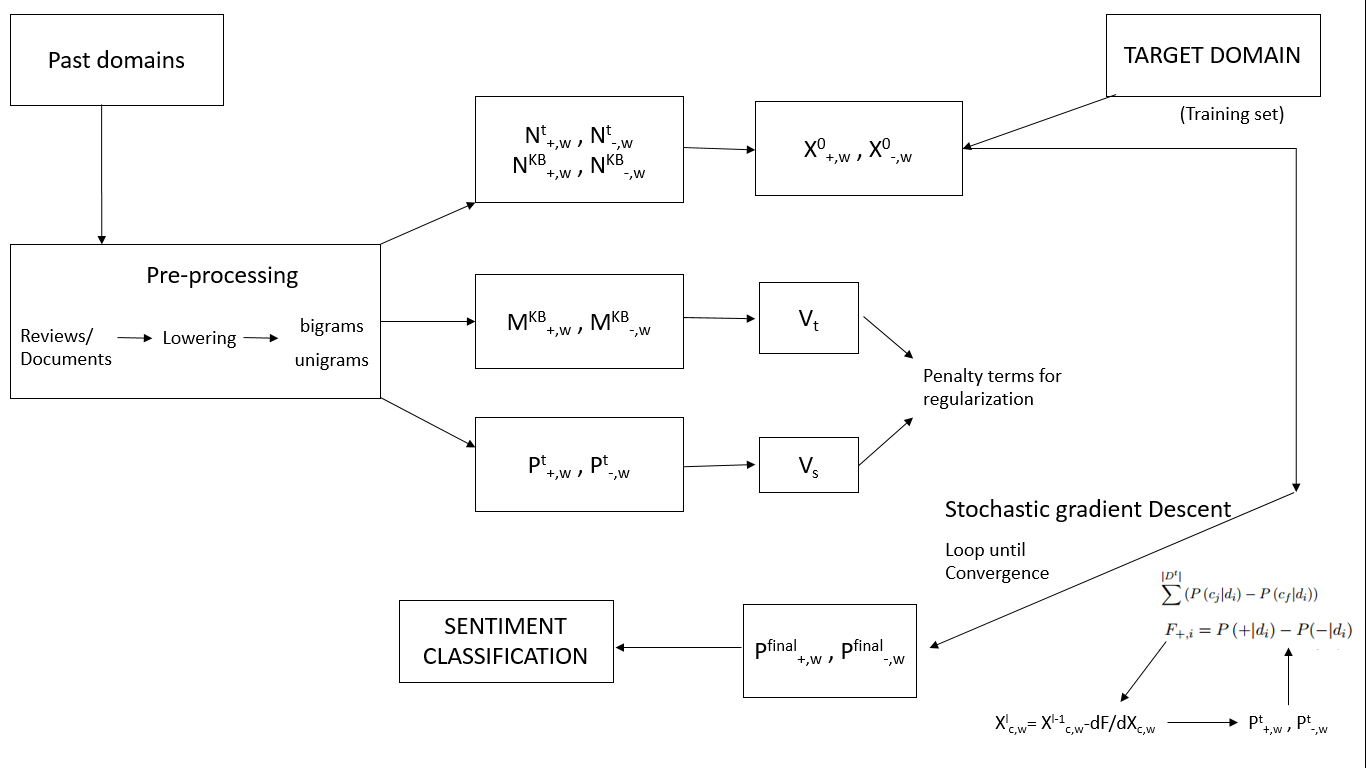
\includegraphics[scale=0.2]{system}
%
%\begin{itemize}
%	\item \textbf{Storing knowledge}: This component is to process the reviews from the past domains and gain the parameters for learning task on the target domain.
%	Since Vietnamese is an isolated language, we follow the maximum entropy approach of Dinh and Vu~\cite{DDien-VThuy:2006} to segment each document on the Vietnamese dataset.
%	The segmentation task can help better modeling the sentiment adjectives which often contains two or more syllables, hence, provide a better vocabulary set for classification on Vietnamese using unigram feature.
%	On both English and Vietnamese dataset, each review is tokenized into unigrams and bigrams to help us experiment both cases.
%	After the text processing tasks, the system will try to extract the knowledge that will be used to optimize the classifier on the target domain.
%	The main types of knowledge consists of:

\section{Experimental Results}

\subsection{Dataset}

% Mo ta chung ve cac dataset se su dung trong thi nghiem
% In this study, we use two datasets, which are ...
% The first ...
% The second ...
In this study, we used two datasets for sentiment classification, one is Vietnamese and the other is English. 
The English one has been used by Chen et al.~\cite{chen-ma-liu:2015:ACL-IJCNLP} for lifelong learning, in which there are 20,000 product reviews from Amazon divided into 20 domains.
The Vietnamese dataset was also crawled from an e-commerce website, Tiki.vn . %, with consumer reviews on 17 products. 
The two datasets can contribute great values to different tasks of cross-domain sentiment analysis on both languages. 
%total number of reviews, all contain Vietnamese tone marks, do not use emoticons included
% Data for this study were retrospectively collected from ...
% The small size of the dataset meant that it was not possible to ...

\textbf{Labeled Vietnamese reviews} For this study, we crawled the reviews from Tiki.vn, which is a large e-commerce website with quality reviews from the customers.
It is a large corpus of 17 diverse domains or products and a total of 15,394 product reviews, but we selected a group of 10 with a fair amount of negative reviews for experiments (including 13,652 reviews), which we name ``A Community Resource for sentiment analysis on Vietnamese'' (CRSAVi).
This selection not only helped reduce the imbalanced distribution, but also committed enough lexical resources for creating a classifier.
We followed the previous works~\cite{blitzer-dredze-pereira:2007:ACLMain,pang-lee-vaithyanathan:2002:EMNLP02} to treat reviews with more than 3 star as positive reviews, equal to 3 star as neutral and fewer than 3 star as negative ones.
The number of positive, neutral and negative reviews are shown as in the table~\ref{table:Table CRSAVi}:

\begin{table}[htb]
\centering
\caption{Names of 10 domains and the number of positive, neutral and negative reviews}
\begin{tabular}{|L{5cm}|R{1.5cm}|R{1.5cm}|R{1.5cm}|}%R{1cm}|R{1cm}|}
	\hline
	\textbf{Product} &  \textbf{Positive} & \textbf{Neutral} & \textbf{Negative}  \\
	\hline
	TrangDiem(Cosmetics) &	3,629&	792&	154\\
	Dungcuhocsinh(Tools for students) &	1,803&	164&	37\\
	Sanphamvegiay(Papers) &	1,778&	144&	34\\
	Butviet(Pens and pencils) &	1,044&	125&	28\\		
	Dodungnhabep(Kitchen) &	987 &	100&	24\\		
	DauGoi(Shampoo) &	347 &	59&	18\\
	Tainghe(Headphones) &	698&	90&	18\\
	DoDungChoBe(Baby)	&658	&61	&14\\
	Filehosobiahoso(Files)	&157	&47	&14\\
	Phukiendienthoaimaytinhbang(Accessories)	&583	&32	&13\\
%	Nuochoa(Perfume)	&207	&21	&10\\
%	Thietbilamdep(Beauty equipment)	&127	&16	&8\\
%	Butxoaxoakeo(Eraser)	&311	&43	&7\\
%	Mayxaymayep(Grinders)	&395	&38	&7\\
%	Binhdunsieutoc(Kettle)	 &107	&13	&5\\
%	Dungcuanuong(Dining substances)	&114	&19	&5\\
%	TranhDongHo(Dong Ho paintings)	&274	&10	&5\\
	\hline
	Total (13,652 reviews) & 11,684 &	1,614 &	354	 \\
	\hline
\end{tabular}

\label{table:Table CRSAVi}
\end{table}

It is noted that the all product reviews from Tiki was checked by the website administrators before publishing, which helps guarantee low rate of low quality reviews from online users.
In fact, all of them contain Vietnamese tone marks, some contain emoticons. 
%However, for this study, we do not use the emoticons included, only the unigrams and bigrams are used.
On our dataset, the average unigram per document on each domain varies from 66 to just above 75 unigrams.
The information packed in a single review in our dataset consists of the product name, author name, rating, headline, bought-already, time of review and details.
From the table~\ref{table:Table CRSAVi}, it can be seen that the proportion of negative class among the dataset is only around 2.6\%.
%Compared to some other datasets for cross-domain sentiment classification, ours express the real life situation where the number of reviews among domains are quite variant.
As that being said, to experiment lifelong learning, a mass of reviews among multiple product types are required, although there is no Vietnamese sentiment dataset that can meet the requirements.
Although different types of products are crawled for the task and Tiki has a great deal of book reviews, CRSAVi does not include books because most of the book reviews mention the book content, not the overall quality like other products.

%how we pick a group for experiments
Because the difference between the number of reviews across domains might result in the efficiency of the system, for each experiment, we selected randomly a maximum amount of 100 reviews each class on each domain to conduct the experiments. 
%This selection also reduce the imbalanced distribution between positive and negative classes in each domain. 
%From the total of 17 domains, to have a reasonable distribution of negative class on each set, we selected a group of 10 domains which have the most negative reviews.
%This group contains products which have equally and more than 13 negative reviews. 

%For this study, we experimented on both groups, which would show different results due to the distribution and number of reviews across products.

\textbf{Labeled English reviews} The corpus from Chen et al.~\cite{chen-ma-liu:2015:ACL-IJCNLP} was utilized to compare directly to their lifelong learning approach in English sentiment classification.
The corpus contains reviews of 20 different products crawled from Amazon.
The experiments were on a dataset which has a reasonable proportion of negative reviews across domains, varies from 11.97 to 30.51\% .

\subsection{Evaluation Metrics}

The evaluation method used is 5-fold cross validation.
While dividing a domain into groups, we tried to keep the class distribution to avoid the case of no negative review on a segment due to the small proportion of negative class mentioned above.
F1-measure on negative and positive class in types of Micro-average and Macro-average are applied.
%For Vietnamese dataset, we compare the macro-average and micro-average of F1-score on negative class because the imbalanced distribution makes it harder to classify. 

\subsection{Baseline}

Our method is compared to VietSentiWordnet by Vu et al~\cite{vu2014building}.
The approach uses a dictionary which contains a list of segmented words or phrases in Vietnamese that express sentiment.
For each word or phrase, the dictionary provides corresponding positive and negative score.
For each document, the score is evaluated by summing up all (positive score - negative score) of all sentiment words or phrases that are available in the dictionary.
if the score is positive, the document is labeled as positive and vice versa.
It is noted that VietSentiWordnet can only work on a single domain data.

In English, we compare our proposed method to Chen et al.~\cite{chen-ma-liu:2015:ACL-IJCNLP} to illustrate the benefits of our approach on lifelong learning.

\subsection{Bigram feature improves the classification on English dataset}
We compare our result to the original lifelong learning approach of Chen et al.~\cite{chen-ma-liu:2015:ACL-IJCNLP}(LSC) on the balanced class distribution.
We created a balance dataset of 200 reviews (100 positive and 100 negative) in each domain dataset for this experiment.
On balanced class distribution, how the accuracy is improved is expressed as in table~\ref{table:Table en balanced}
\begin{table}[htb]
\centering
\caption{Accuracies on English balanced distribution over 20 domains}
\begin{tabular}{|C{3cm}|C{3cm}|C{3cm}|}
	\hline
	\textbf{LSC}  & \textbf{LSC-bag-of-bigram} & \textbf{LSC-bigram}\\
	\hline
	83.34 & \textbf{85.92} & 85.44 \\
	\hline
\end{tabular}

\label{table:Table en balanced}
\end{table}

Our method exceeds LSC to get to a high of 85.92\%.
This improvement confirms the results of Wang et al.~\cite{wang-manning:2012:ACL2012short} and proves that the use of bigram and bag-of-bigram features also improve the performance on cross-domain sentiment classification.

\subsection{Vietnamese cross-domain sentiment classification}
We compare our proposed method in different settings to the baseline method on the Vietnamese dataset. 
The average F1-score for the positive class is not shown because being the majority class makes the classifiers perform well and do not show much difference between multiple settings, although they all perform better than VietSentiWordnet.
%In this group, we first 
Table~\ref{table:Table vi VSenti vs uni} compares VietSentiWordnet(VSWN) to our proposed method (lifelong learning for Vietnamese sentiment classification-now called LLVi) using unigram feature with segmentation (LLVi-
uni) and without segmentation (LLVi-uniWS). 

The LLVi with unigram feature (no segmentation) which also counts emoticons (LLVi-e) is also compared.
\begin{table}[htb]
	\centering
\caption{Macro,micro average F1-score of the negative class on CRSAVi}
	\begin{tabular}{|R{1.5cm}|R{1.6cm}|R{1.6cm}|R{1.6cm}|R{2.1cm}|}
		\hline
		{}&\textbf{VSWN} & \textbf{LLVi-uni} & \textbf{LLVi-e} & \textbf{LLVi-uniWS}\\
		\hline
		Macro F1 & 33.21 & 47.19 & \textbf{51.20} & 50.87\\
		\hline
		Micro F1 & 40.85 & 61.33 & \textbf{62.12} & 61.93 \\
		\hline
	\end{tabular}

\label{table:Table vi VSenti vs uni}
\end{table}

The table~\ref{table:Table vi VSenti vs uni} has obviously shown that while segmentation task helps improving the performance on lifelong learning with unigram feature.
For example, the word ``tuy\_nhiên'' (however) can classify well in our dataset, but cannot be leveraged effectively without segmentation.
%The emoticons also play a huge role in sentiment classification whereas they improves the performance slightly.
However, lifelong learning with emoticons still performs slightly better.
The two emoticons ``:('' and ``:)'' provides significantly biased probability thus become good classifiers.
The table~\ref{table:Table vi VSenti vs uni} also confirms that the lifelong learning approach has a huge advantage over VietSentiWordnet, which can only work on the target domain.

%uni vs bi vs bob ||h uniws vs bi ws vs bobws
Table~\ref{table:Table vi bibob} compares the performance is a collection of lifelong learning approaches with different features applied. 
The group includes LLVi-uni, LLVi with bigram feature (LLVi-bi), LLVi with bag-of-bigram feature (LLVi-bb) in two settings, segmentation and without segmentation.
\begin{table}[htb]
	\centering
	\caption{Macro, micro average F1-score on negative class with Vietnamese dataset, unigram vs bigram vs bag-of-bigram. Unit: \%}
	\begin{tabular}{|R{1.5cm}|R{2.1cm}|R{1.6cm}|R{1.6cm}|R{1.6cm}|}
		\hline
		 & & \textbf{LLVi-uni} & \textbf{LLVi-bi} & \textbf{LLVi-bb} \\
		\hline
		\multirow{2}{*}[-0.5em]{macro F1} & no segmentation & 47.19 & 56.10  & 60.56 \\
		\cline{2-5}
		 & with segmentation & 50.87 & 64.37  & \textbf{65.85}\\
		\hline
		\multirow{2}{*}[-0.5em]{micro F1} & no segmentation & 61.33 & 56.52 & \textbf{66.27} \\
		\cline{2-5}
		 & with segmentation & 61.93 & 61.53 & 60.59 \\
		\hline
	\end{tabular}
	
	\label{table:Table vi bibob}
\end{table}
Similar to English, using bigram and bag-of-bigram features make a huge improvement to the performance compared to using unigram feature only. 
With segmentation combined, the lifelong learning using unigram feature improves significantly, while it does not have clear impact on lifelong learning with bigram and bag-of-bigram features.
'cực\_kỳ tốt'(extremely good), 'khó chịu'(frustrating), 'rát da'(burning skin sensation), 'chẳng mê'(cannot love) are examples of how using bigram performs better.


\section{Conclusion}
In this paper, we have presented our method that uses lifelong learning for cross-domain sentiment classification on English and Vietnamese. 
Experimental results on both corpus showed that:
\begin{itemize}
	\item Lifelong learning approach is effective for cross-domain sentiment classification in Vietnamese as well as in English.
	\item Incorporating bigram and bag-of-bigram features into lifelong learning improved the performance of the system.
	\item Emoticons and word segmentation made a slight improvement in sentiment classification on the Vietnamese dataset.
\end{itemize}

There is abundant room for further progress of our work.
We would like to further exploit the sentiments from emoticons due to the high rate of occurrences of these in our dataset. 
Besides, future work could be focused on another collection of reviews with different qualities and different types of products to verify our proposed method.

\section*{Acknowledgments}
This research is supported by research funding from Honors Program, University of Science, Vietnam National University - Ho Chi Minh City.


\bibliographystyle{splncs} 

\bibliography{ref}

\end{document}